\section{Results}
\label{sec:results}





\subsection{Measuring $\gamma(\Delta)$}

\NS{Operations plot}

\begin{figure}
    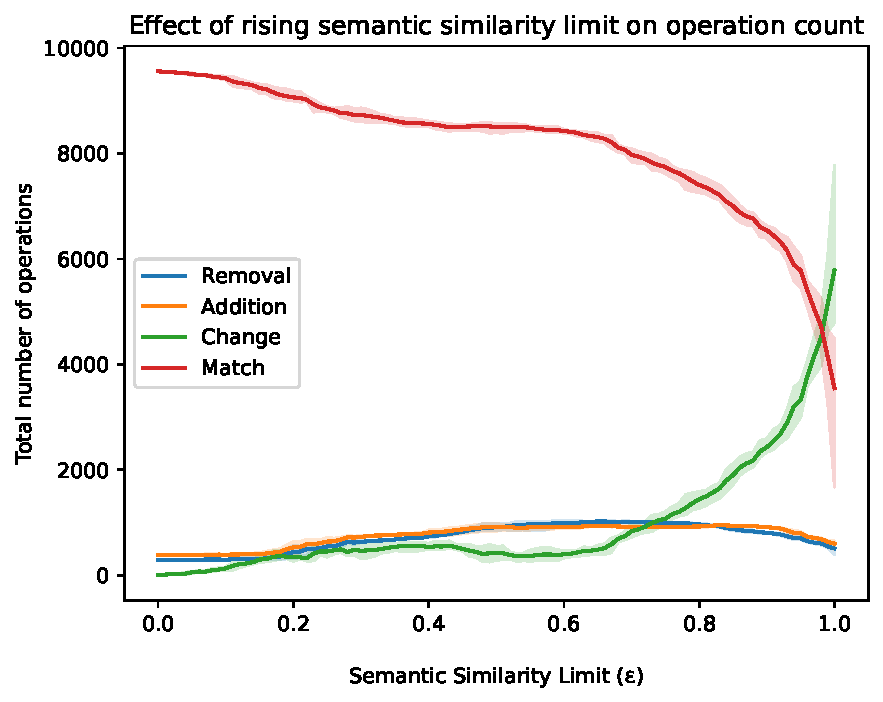
\includegraphics[width=\linewidth]{code/img/operation_count.pdf}
    \caption{The average distance between the 38 experimental ATs per semantic similarity limit}
    \label{img:operation-count}
\end{figure}

\subsection{Finding optimal $\epsilon$}

In Figure~\ref{img:similaritylimits}, we can see the effect of rising semantic similarity limit ($\epsilon$) on the average distance between each of attack tree 1 ($n=38$). Additionally, we can see the normalized Levenshtein distance plotted against the same semantic similarity limits. Finally, we can see the traditional Zhang and Shasha edit distance (based on string equivalence), which is unaffected by a similarity limit.

\begin{figure}
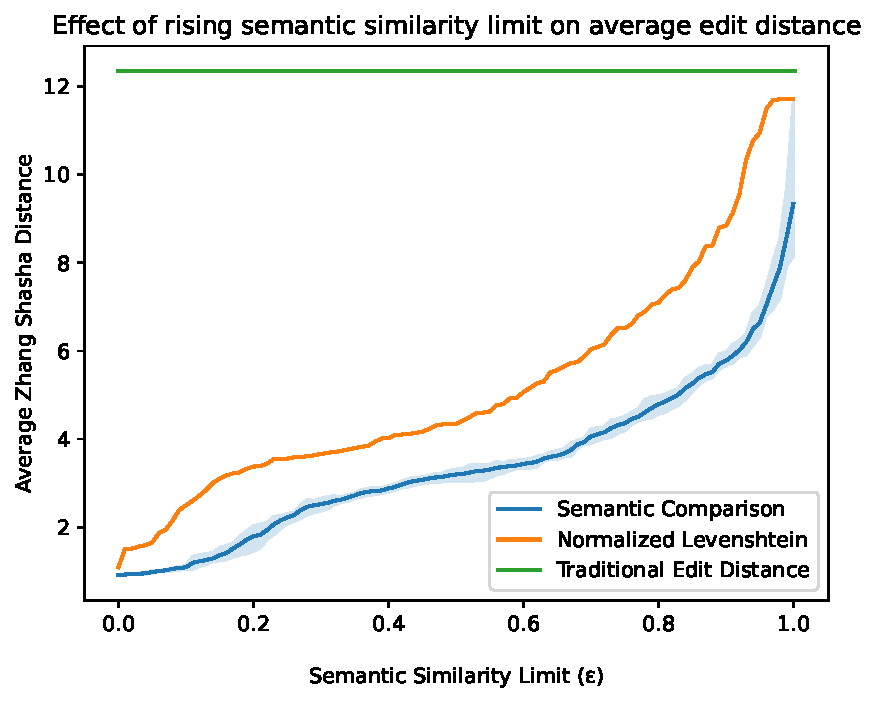
\includegraphics[width=\linewidth]{code/img/similaritylimits2.pdf}
\caption{The average distance between the 38 experimental ATs per semantic similarity limit}
\label{img:similaritylimits}
\end{figure}

\NS{Operations plot}


\section{Effect of node flipping}

\NS{plot showing average distance between 38 ATs with and without node flipping}

